\section{The Data}
\label{sec:data}

\qquad There are 3 datasets provided, \textit{lingData}, \textit{lingLocation} and \textit{question\_data}. 47471 people from all over the country were surveyed on 122 questions, of which only 67 questions are used for our analysis. 
In dataset \textit{lingData}, each row is one individual with features \textit{ID}, \textit{CITY}, \textit{STATE}, \textit{ZIP}, \textit{lat} (latitude), \textit{long} (longitude) and their responses to questions. 
\textit{ID} is the individual index while \textit{CITY}, \textit{STATE}, \textit{ZIP}, \textit{lat}, \textit{long} describe the location. Dataset \textit{lingLocation} aggregates Dataset \textit{lingData} by put people with the same \textit{lat}, \textit{long} and responses together. Dataset \textit{question\_data} gives the concrete content of each question (Refer to \href{http://dialect.redlog.net/index.html}{Harvard Dialect Survey} for more questions).

\subsection{Data quality and cleaning}
\qquad We check the data quality and process some necessary data cleaning to make it tidy enough for further exploration and analysis. To figure out the geographic patterns of dialects, we decide to use \textit{county} as the basic unit with the belief that people in the same county are supposed to share the same cultures, customs and dialects. One way to assign each person to the county he locates in is to use \textit{FIPS county code}. We first need to match the \textit{ZIP code} offered in \textit{lingData} to \textit{FIPS county code} downloaded online. However, 5234 people's \textit{ZIP}s do not match any \textit{FIPS} approximately due to the incompleteness of our \textit{ZIP2FIP} file. We eventually decided to make use of each participant's \textit{lat} and \textit{long} to figure out his corresponding \textit{county}. During the procedure, we added another two fields to each individual, \textit{COUNTY} (merging both the state and the county by ',') and \textit{group} (the index of \textit{COUNTY}). The following are steps of data cleaning:

\begin{enumerate}
\begin{figure}[t!]
    \centering
    \begin{subfigure}[t]{0.49\textwidth}
        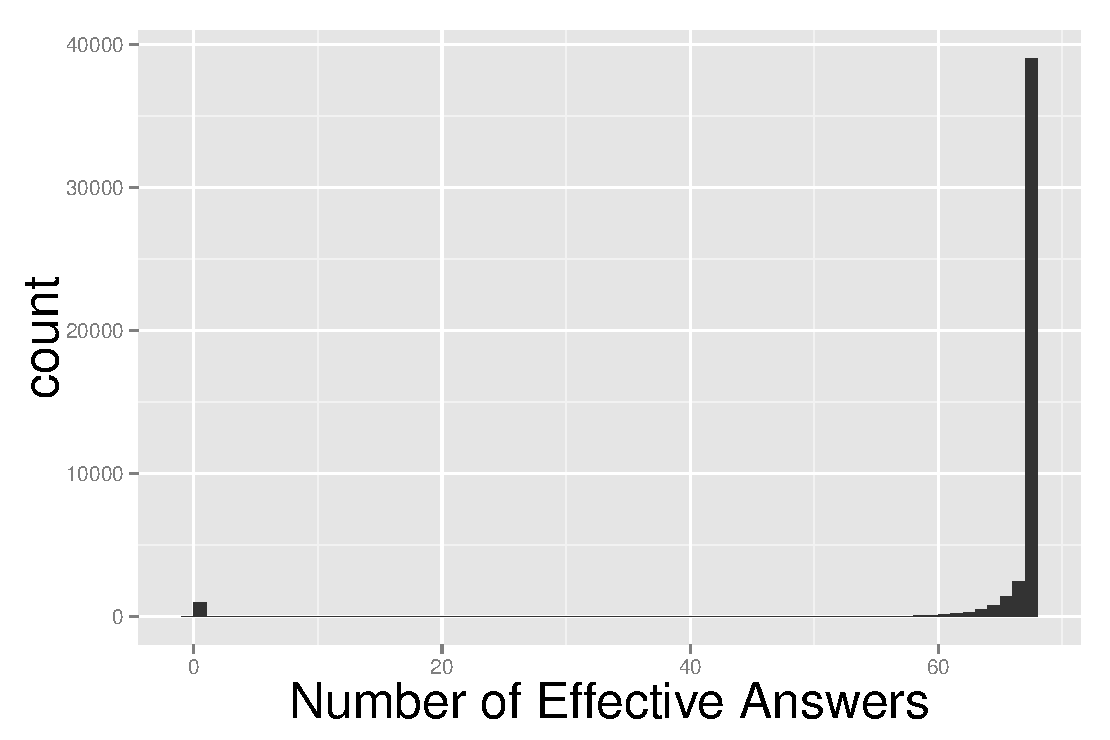
\includegraphics[width=1\textwidth]{fig/Anw_distri_all.pdf}
        \caption{all}
    \end{subfigure}
    \begin{subfigure}[t]{0.49\textwidth}
        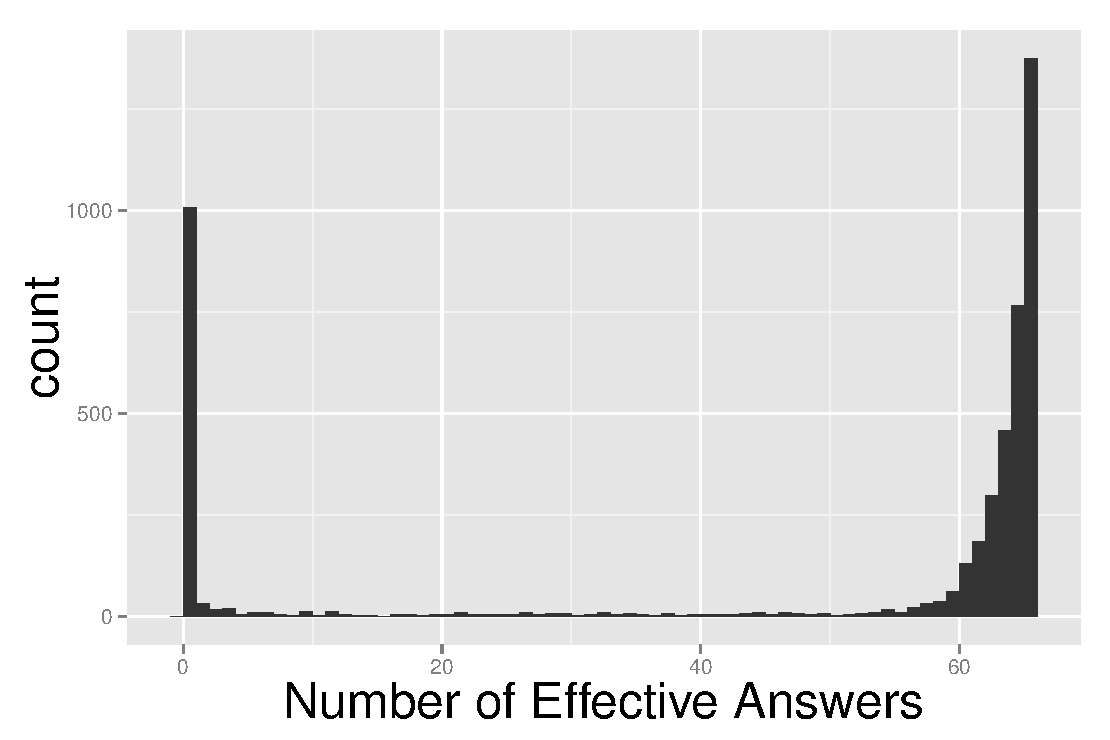
\includegraphics[width=1\textwidth]{fig/Anw_distri_65.pdf}
                \caption{no more than 65}
    \end{subfigure}
    \caption{\textbf{The distribution of people with different numbers of effective responses.} \textbf{(a)} All people. \textbf{(b)}  People who had no more than 65 responses.} 
\end{figure}

\item Our focus is on the mainland of the U.S., thus areas outside the American mainland are excluded, like Alaska, Hawaii. In this step, 1232 people are not in the range. There remain 46239 individuals.

\item There are some missing responses for a few people due to erroneous records or that they were not willing to response the corresponding question. People with few responses are of little use to our analysis, thus need to be excluded. After having a look at the distribution of people with different effective responses (See \textbf{Figure xxx}), we selected people who had responded to at least 60 questions, with little loss of information. In this step, there remain 44683 people.

\item As mentioned above, each individual's county is figured out by using their \textit{lat} and \textit{long}. However, some people cannot be matched to any counties, thus should be removed from the datasets. During the matching process, we add both the name of count (\textit{COUNTY}) and the county index (\textit{group}) each person. In this step, there remain 43401 people.

\item Some counties have more than one count indexes, which may be used to differentiate the direction of counties, e.g. North Berkeley and South Berkeley. Without much loss of information, we remove such repetitions. In this step, there remain 43266 people.

\item Since the question response belongs to categorical data and cannot be compared directly between questions. We need to transform each person's response into a binary format. For example, if one question has 4 responses one person chose the second option, his response is expressed as $(0,1,0,0)$. Finally, each person has a response vector of length of 468 (the sum of the number of responses times the number of its associated options), each loading is an indicator if he chose this option. Here we get a response matrix with dimension of 43266 by 468 on individual level.

\item We also aggregate the response matrix on individual level into county level with the consideration that the county is our basic unit for dialect geography. We simply take an average of the response vectors among people in the same county. The dimension of the response matrix on county level is 2362 by 468. 

\end{enumerate}

\begin{figure}[t!]
    \centering
    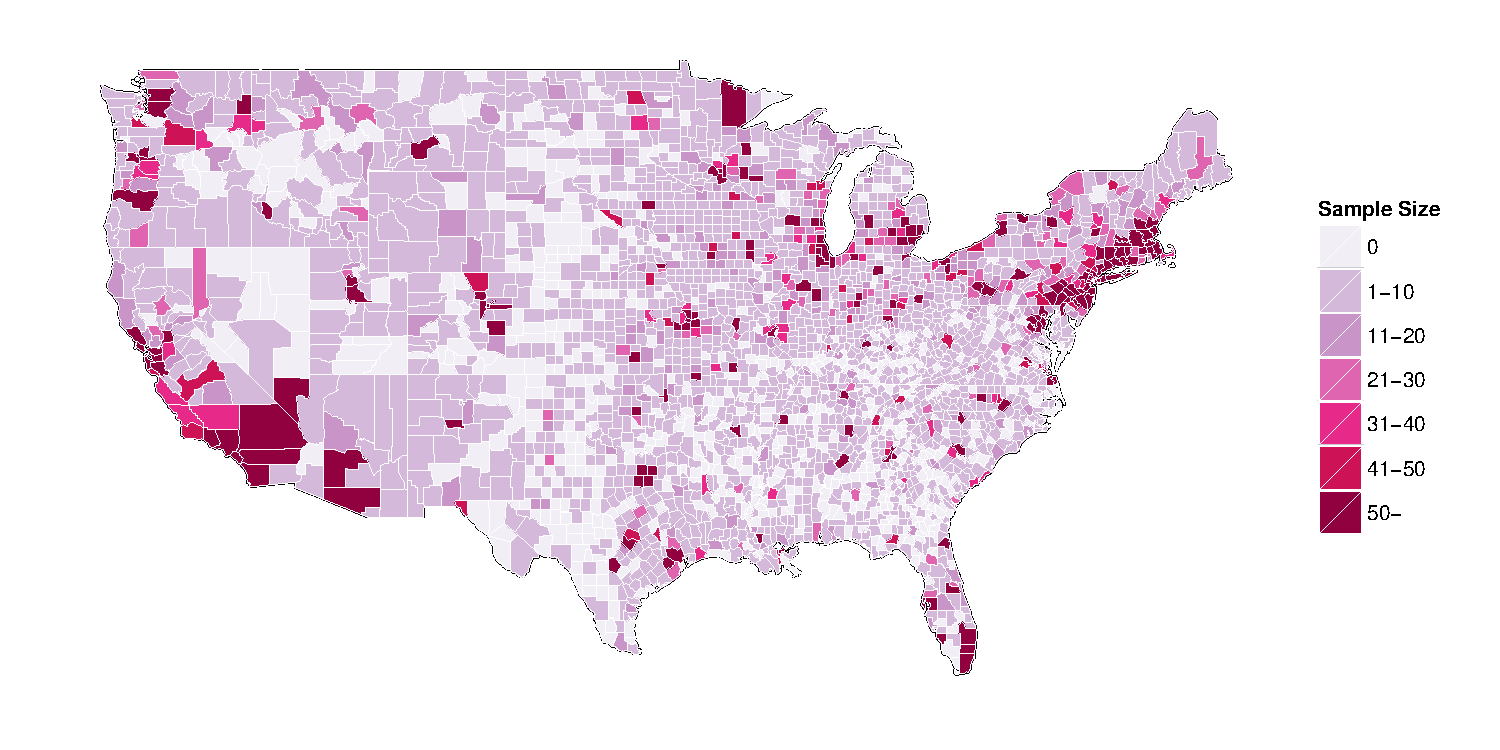
\includegraphics[width=1\textwidth]{fig/Map_size.pdf}   
    \caption{\textbf{The distribution of sample size on counties} 2362 counties have people who taken part in the survey while 713 counties have no surveyed individuals.} 
\end{figure}

\qquad We only make use of Dataset \textit{lingData} and match the counties by ourselves in case of the inaccuracy of the existing \textit{CITY} and \textit{ZIP} information. The data possesses high quality so that we do not make too many efforts for tidying it. But the survey design receives the doubt that people were not surveyed uniformly from all over the countries. 713 counties do not have people who taken part in the survey (See \textbf{Figure xxx}).

